\documentclass[conference]{IEEEtran}

\usepackage{cite}

\linespread{0.9}

% Encoding and Language
\usepackage[utf8]{inputenc}
\usepackage[english]{babel}

% Spacing
\usepackage{xspace}

% Images
\usepackage{graphicx}
\usepackage{subcaption}
\graphicspath{{./img/}}
\DeclareGraphicsExtensions{.pdf,.jpeg,.png}

% Tables
\usepackage{booktabs}
\usepackage{multirow}

% Enumerations
\usepackage[inline]{enumitem}
\renewcommand*\descriptionlabel[1]{\hspace\labelsep\itshape #1}

% Units
\usepackage{amssymb}
\usepackage{siunitx}
\DeclareSIUnit{\nothing}{\relax}

% URLs
\usepackage{url}

% Hyper References
\usepackage[hidelinks=true]{hyperref}
\usepackage{nameref}

% Acronyms
\usepackage[acronym,nowarn]{glossaries}
\glsdisablehyper
%=============================================================================
% Computer Architecture
%=============================================================================

% CPU
\newacronym{cpu}{CPU}{Central Processing Unit}
	\newcommand{\cpu}{\gls{cpu}\xspace}
	\newcommand{\cpus}{\glspl{cpu}\xspace}
\newcommand{\ccluster}{Compute Cluster\xspace}
\newcommand{\cclusters}{Compute Clusters\xspace}
\newcommand{\iocluster}{I/O Cluster\xspace}
\newcommand{\ioclusters}{I/O Clusters\xspace}
\newacronym{pe}{PE}{Processing Element}
	\newcommand{\pe}{\gls{pe}\xspace}
	\newcommand{\pes}{\glspl{pe}\xspace}
\newacronym{rm}{RM}{Resource Manager}
	\newcommand{\rman}{\gls{rm}\xspace}
	\newcommand{\rmans}{\glspl{rm}\xspace}

\newacronym{dram}{DRAM}{Dynamic Random Access Memory}
	\newcommand{\dram}{\gls{dram}\xspace}
\newacronym{sram}{SRAM}{Static Random Access Memory}
	\newcommand{\sram}{\gls{sram}\xspace}

% NoC
\newacronym{noc}{NoC}{Network-on-Chip}
	\newcommand{\noc}{\gls{noc}\xspace}
	\newcommand{\nocs}{\glspl{noc}\xspace}
\newacronym{cnoc}{C-NoC}{Control NoC}
	\newcommand{\cnoc}{\gls{cnoc}\xspace}
\newacronym{dnoc}{D-NoC}{Data NoC}
	\newcommand{\dnoc}{\gls{dnoc}\xspace}

% MIMD
\newacronym{mimd}{MIMD}{Multiple Instruction Multiple Data}
	\newcommand{\mimd}{\gls{mimd}\xspace}

% Kalray
\newcommand{\mppa}{Kalray MPPA-256\xspace}

% LWs
\newcommand{\lw}{lightweight manycore\xspace}
\newcommand{\Lw}{Lightweight manycore\xspace}
\newcommand{\lws}{lightweight manycores\xspace}
\newcommand{\Lws}{Lightweight manycores\xspace}

% Epiphany
\newcommand{\epiphany}{Adapteva Epiphany\xspace}

% Intel
\newcommand{\scc}{Intel Single-Cloud Computer\xspace}

% SPM
\newacronym[longplural={Scratchpad Memories}]{spm}{SPM}{Scratchpad Memory}
	\newcommand{\spm}{\gls{spm}\xspace}
	\newcommand{\spms}{\glspl{spm}\xspace}

% OpTiMSoC
\newcommand{\optimsoc}{OpTiMSoC\xspace}

% Sunway
\newcommand{\taihulight}{Sunway SW26010\xspace}

% Tilera
\newcommand{\tilegx}{Tilera TILE-Gx100\xspace}
\newcommand{\tilepro}{Tilera TILE64\xspace}

%=============================================================================
% Runtime Systems
%=============================================================================

\newcommand{\runtimesys}{runtime systems\xspace}

% MPI
\newacronym{mpi}{MPI}{Message Passing Interface}
	\newcommand{\mpi}{\gls{mpi}\xspace}

% OpenMP
\newcommand{\openmp}{OpenMP\xspace}

% OpenSHMEM
\newcommand{\openshmem}{OpenSHMEM\xspace}

% PGAS
\newacronym{pgas}{PGAS}{Partitioned Global Address Space}
	\newcommand{\pgas}{\gls{pgas}\xspace}

% MPB
\newacronym{mpb}{MPB}{Message Passing Buffer}
	\newcommand{\mpb}{\gls{mpb}\xspace}

%=============================================================================
% Operating Systems
%=============================================================================

% DMA
\newacronym{dma}{DMA}{Direct Memory Access}
	\newcommand{\dma}{\gls{dma}\xspace}
	\newcommand{\dmas}{\glspl{dma}\xspace}
\newacronym{rma}{RMA}{Remote Memory Access}
	\newcommand{\rma}{\gls{rma}\xspace}

% IPC
\newacronym{ipc}{IPC}{Inter-Process Communication}
	\newcommand{\ipc}{\gls{ipc}\xspace}

% Microkernel
\newcommand{\microkernel}{\textit{microkernel}\xspace}

% Multikernel
\newcommand{\multikernel}{\textit{multikernel}\xspace}

% POSIX
\newacronym{posix}{POSIX}{Portable Operating System Interface}
	\newcommand{\posix}{\gls{posix}\xspace}

% API
\newacronym{api}{API}{Application Programming Interface}
	\newcommand{\api}{\gls{api}\xspace}
	\newcommand{\apis}{\glspl{api}\xspace}

% OSes
\newacronym[plural=OSes,firstplural=Operating Systems (OSes)]{os}{OS}{Operating System}
	\newcommand{\os}{\gls{os}\xspace}
	\newcommand{\oses}{\glspl{os}\xspace}

% Nanvix
\newcommand{\nanvix}{Nanvix\xspace}

%=============================================================================
% LIBMPI
%=============================================================================

% LwMPI
\newcommand{\lwmpi}{LWMPI\xspace}

% libmpi
\newcommand{\libmpi}{\texttt{LibMPI}\xspace}

% mputil
\newcommand{\mputil}{\texttt{MPUtil}\xspace}

% MPI_Send
\newcommand{\mpisend}{\texttt{MPI\_Send}\xspace}

% MPI_Recv
\newcommand{\mpirecv}{\texttt{MPI\_Recv}\xspace}

%=============================================================================
% Institutions
%=============================================================================

% PUC Minas
\newacronym{pucminas}{PUC Minas}{Pontifícia Universidade Católica de Minas Gerais}
	\newcommand{\pucminas}{\gls{pucminas}\xspace}

% UFSC
\newacronym{ufsc}{UFSC}{Universidade Federal de Santa Catarina}
	\newcommand{\ufsc}{\gls{ufsc}\xspace}

% UGA
\newacronym{uga}{UGA}{Université Grenoble Alpes}
	\newcommand{\uga}{\gls{uga}\xspace}

% CNPq
\newacronym{cnpq}{CNPq}{Conselho Nacional de Desenvolvimento Tecnológico}
	\newcommand{\cnpq}{\gls{cnpq}\xspace}

%=============================================================================
% Nanvix
%=============================================================================

% IKC
\newacronym{ikc}{IKC}{Inter Kernel Communication}
	\newcommand{\ikc}{\gls{ikc}\xspace}

% Mailbox
\newcommand{\mailbox}{\textit{mailbox}\xspace}
\newcommand{\mailboxes}{\textit{mailboxes}\xspace}

% Portal
\newcommand{\portal}{\textit{portal}\xspace}
\newcommand{\portals}{\textit{portals}\xspace}

% Sync
\newcommand{\sync}{\textit{sync}\xspace}
\newcommand{\syncs}{\textit{syncs}\xspace}

%=============================================================================
% MISC
%=============================================================================

% Megabyte
\newacronym{megabyte}{MB}{Megabyte}
	\newcommand{\megabyte}{\gls{megabyte}\xspace}
	\newcommand{\megabytes}{\gls{megabyte}\xspace}

\newacronym{upc}{UPC}{Unified Parallel C}
	\newcommand{\upc}{\gls{upc}\xspace}

%=============================================================================
% Writing
%=============================================================================

% Abbreviations
\newcommand{\ie}{i.e.,\xspace}
\newcommand{\eg}{e.g.,\xspace}
\newcommand{\etal}{\textit{et al.}\xspace}
\newcommand{\hseparator}{$\cdot$\xspace}

\makeglossaries

\sloppy

\begin{document}

\author{\IEEEauthorblockN{João Fellipe Uller}
\IEEEauthorblockA{\textit{Universidade Federal de Santa Catarina (UFSC)}\\
Florianópolis, Brazil \\
joao.f.uller@grad.ufsc.br}
}

\title{A performance evaluation using an MPI library over the communication infrastructure of Nanvix}

\author{\IEEEauthorblockN{João Fellipe Uller}
\IEEEauthorblockA{\textit{Universidade Federal de Santa Catarina (UFSC)}\\
Florianópolis, Brazil \\
joao.f.uller@grad.ufsc.br}
}

\maketitle

\begin{abstract}
	The performance and energy efficiency provided by \lws is
	undeniable. However, the lack of rich and portable support for
	these processors makes software development challenging. In this work,
	we propose a portable and lightweight
	MPI library (\lwmpi) designed from scratch to
	cope with the intricacies of \lws. We integrated \lwmpi
	into a distributed OS that targets these processors
	and evaluated it on the \mppa processor. Results obtained with three applications
	from a representative benchmark suite unveiled that \lwmpi achieves similar
	performance scalability in comparison with a low-level vendor-specific API narrowed
	for MPPA-256, while exposing a richer programming interface.
\end{abstract}

\begin{IEEEkeywords}
	lightweight manycores, runtime systems, MPI, high-performance computing
\end{IEEEkeywords}

\glsresetall
               % 0.5 p
\section{Introduction}
\label{sec:introduction}

	% Context: Lightweight Manycore Processors
	Lightweight manycore processors emerged to address demands on
	high-performance and energy efficiency~\cite{Francesquini2015}.
	On the one hand, to deliver high-performance and scalability, these
	processors rely on a distributed memory architecture and a rich
	\noc.  On the other hand, to achieve energy
	efficiency, they are built with simple low-power \mimd
	cores and \spms  with no hardware coherency
	support.  Moreover, they exploit heterogeneity
	by combining cores with different capabilities.
	Some industry-successful examples of \lws are the
	\mppa~\cite{DeDinechin2013-2} and the \epiphany~\cite{Olofsson2016}.

	% Motivation #1: Architectural Challenges
	However, while the aforementioned architectural features make lightweight
	manycores so interesting, they also introduce several challenges
	in software programmability.  For instance, the \textit{distributed
	memory architecture} requires a non-trivial software design where the
	data should be explicitly fetched from remote memories to local
	ones to be manipulated~\cite{Francesquini2015}.  Furthermore, the
	\textit{small amount of on-chip memory} demands software to
	explicitly tile the working data set into chunks and locally
	manipulate them one at a time~\cite{Souza2017}.
	Finally, the rich \noc exposes mechanisms for asynchronous programming
	to overlap communication with
	computation~\cite{Hascoet2017}; and hand-operated routing to
	guarantee uniform communication latencies.

	% Motivation #2: Software Development Support
	Currently, two approaches are employed to address programmability
	challenges in \lws: \oses~\cite{Kluge2014,
	Asmussen2016, Penna2019-3} and baremetal
	\runtimesys~\cite{Dinechin2013-1, Varghese2014, Richie2017}. The
	former is meant to bridge critical programmability gaps imposed by hardware
	intricacies.  The latter aims to expose a rich, performance-oriented
	programming environment, narrowed to the underlying architecture.
	While these two approaches are effective for some use cases, they
	have a significant duality drawback. Application development directly
	on top of \os interfaces yields to software portability, but the actual
	programming interface provided is
	complex and delay the software development process.  In contrast,
	baremetal and vendor-specific \runtimesys expose richer interfaces
	that accelerate the development process, but they exclusively concern to
	the software stack ecosystem of a specific lightweight manycore, resulting
	in non-portable applications.

	% The Paragraph: Problem, Hypothesis, Goals and Contributions
	In this work, we present a third proposition, trying to address the programmability and
	portability challenges of \lws, by combining both approaches: a lightweight
	implementation of the \mpi standard (named \lwmpi) on top of \nanvix,
	a \posix-compliant distributed \os that targets \lws~\cite{Penna2019-3}.
	%
	% Evaluation Methodology
	To assess \lwmpi with representative
	computing workloads, we carried out experiments with three applications extracted
	from the CAP Bench suite~\cite{Souza2017}. All experiments were executed on the
	\mppa, a baremetal lightweight manycore. Our results unveiled that \lwmpi delivers
	similar performance scalability when compared
	with a vendor-specific low-level \api for the \mppa, while exposing a richer
	programming interface.

	% Work Structure
	% The remainder of this work is organized as follows.
	% In Section~\ref{sec:related-work} we discuss related works. In
	% Section~\ref{sec:proposal}, we present an architectural overview of \lwmpi.
	% In Section~\ref{sec:evaluation-methodology}, we
	% detail our evaluation methodology and present the \mppa. In
	% Section~\ref{sec:experimental-results},
	% we discuss the experimental results. Finally, in
	% Section~\ref{sec:conclusions}, we draw our conclusions.
           % 1.5 p
\section{Related Work}
\label{sec:related-work}

	Software development for lightweight manycores is challenging
	because it strives in finding the balance between performance and
	programmability. In this context and specifically concerning
	communication, there are two approaches currently employed:
	%
	\begin{enumerate*}[label=(\roman*)]
		\item vendor-specific communication libraries, which expose a
			performance-oriented interface for the underlying
			architecture; and 

		\item industry-standard communication libraries, which provide a
			richer communication interface, in exchange for some
			performance penalty.
	\end{enumerate*}

	Vendor-specific solutions mostly rely on specific features of the
	underlying hardware to deliver performance. For instance,
	synchronous~\cite{Wijngaart2011} and asynchronous~\cite{Clauss2011}
	interfaces are provided on top of \mpb for the \scc. The \mppa features
	both a communication library that shares some similarity
	with \posix~\cite{Dinechin2013-1} and a specific interface for one-sided
	communications~\cite{Hascoet2017}.
	Finally, a specific communication \api is provided for the \epiphany
	processor~\cite{Varghese2014}.

	In contrast, standard communication interfaces benefit from
	extensive improvements and optimizations, being a solid choice
	for programming lightweight manycores. However, to the best of our
	knowledge, all standard communication interfaces ports are built on
	top of low-level primitives and libraries provided by the vendors,
	making it difficult to adapt them to other
	manycore processors. Examples of such solutions are those based on
	the \pgas programming model, such as the \upc port for the
	\scc~\cite{Gamell2012} and the \openshmem implementation~\cite{Ross2016}
	for the \epiphany processor.  Moreover, there have been some efforts on
	providing an \mpi port for \mppa~\cite{Quan2015} and
	\epiphany~\cite{Richie2017}. The former is the closest work to the
	present one, also presenting an implementation from scratch to cope
	with the restrictions of lightweight manycores. The main difference,
	however, is the fact that it is implemented on top of a
	vendor-specific \ipc library, and so, being not portable to other
	processors/architectures. The latter, in addition, does not conform
	with the \mpi standard.

	Overall, both approaches lack in application
	portability. This work takes a step further on providing a
	flexible and extendable implementation of a well-known parallel
	programming standard (\mpi) on top of an open-source \os for
	lightweight manycores (\nanvix), offering a standard high
	performance solution applyable to a broad range of \lws.
           % 1.0 p
\section{LWMPI: Lightweight MPI for Manycores}
\label{sec:proposal}

	% Present LWMPI
	Aiming at better programmability in lightweight manycores,
	we propose \lwmpi\footnote{\lwmpi is available at:
	\url{https://github.com/nanvix/libmpi}}: an \mpi library for these
	processors.
	%
	% Aims (portability, programmability, cope with restritions)
	The design goals that guided the implementation of \lwmpi are:
	%
	\begin{enumerate}[label=(\roman*)]
		\item \textit{portability}: the library should be portable and
			applicable to various \lws; we enable this by designing it
			on top of a \posix-compliant \os (Nanvix);

		\item \textit{compatibility}: the implementation
			must comply with the \mpi specification; it sticks to the
			3.1 version;

		\item \textit{extendability}: it should be possible to add new
			functions or submodules to the implementation with little
			effort; as so, we design it in a tier-based scheme; and

		\item \textit{lightness}: the implementation should be simple and
			lightweight to cope with restrictive resources of \lws; for that,
			we implemented it from scratch, rather than adapting an existing
			heavy-weight solution like
			% OpenMPI~\cite{OpenMPI2020} or
			% MPICH~\cite{MPICH2020}.
			OpenMPI\footnote{OpenMPI website: \url{https://www.open-mpi.org}} or
			MPICH\footnote{MPICH website: \url{https://www.mpich.org}}
	\end{enumerate}


\subsection{\lwmpi Architecture}
\label{sec:libmpi-impl}

	% Justifying partial support
	Currently, \lwmpi implements an initial subset of the \mpi
	specification (version 3.1). We opted for this partial support since
	fully implementing the entire standard would result in a much bigger
	memory footprint, violating the \textit{lightness} design goal.
	%
	% LWMPI architectural overview
	Figure~\ref{figure:libmpi-arch} presents the two-tier approach
	adopted by \lwmpi on top of \nanvix.

	\begin{figure}[t]
		\centering
		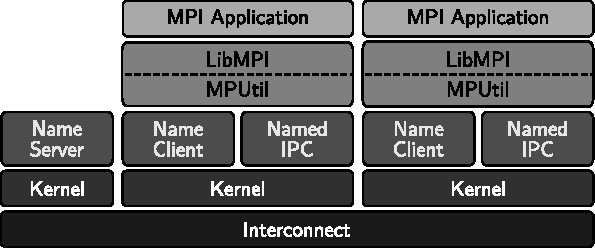
\includegraphics[width=0.9\linewidth]{libmpi}
		\caption{Architectural overview of \lwmpi.}
		\label{figure:libmpi-arch}
		\vspace{-15pt}
	\end{figure}

	The \libmpi tier encapsulates the top-level library and is the
	entry point for user applications.
	%
	% Layer overview
	This layer exposes the library interface and implements the backend
	functions over \mputil. It focuses on filtering
	the input parameters given by the user, performing the
	runtime management and choosing the underlying protocols employed by
	the \mpi calls.
	%
	% Already implemented in LWMPI
	In its current version, our library implements: functions for
	\textit{runtime management}, such as \texttt{MPI\_Init} and
	\texttt{MPI\_Finalize}; support for \textit{communicators} and
	information retrieving, such as \texttt{MPI\_Comm\_rank} and
	\texttt{MPI\_Comm\_size}; support for \textit{groups} of communication
	similarly to communicators;	\textit{error handlers}; and point-to-point
	communication via \mpisend and \mpirecv in the synchronous mode and
	carrying any of the predefined \textit{data types} for the C language.

	% MPUTIL presenting
	The \mputil tier is the middle layer between the overlying library and
	the base \os. Precisely, it is responsible for translating the requests
	from \libmpi to the \nanvix interface. \mputil exposes elementary
	abstractions that support the top-level tier, aiming at keeping the
	library implementation decoupled from the \os interface. It is also
	in this level where the communication protocols used in the \mpi calls
	are implemented.
	%
	% MPUTIL positioning
	To perform these protocols, \mputil relies on the named \ipc
	abstractions exposed by the \textit{Name Service} of the \nanvix
	runtime system, which include
	primitives for fine-grain fixed-size transfers (\mailbox),
	coarse-grain fixed-size transfers (\portal), and
	synchronization points (\sync)~\cite{Souto2020}.

\subsection{Point-to-Point Communication in \lwmpi}
\label{sec:lwbmpi-sendrecv}

	\begin{figure}[b]
		\centering
		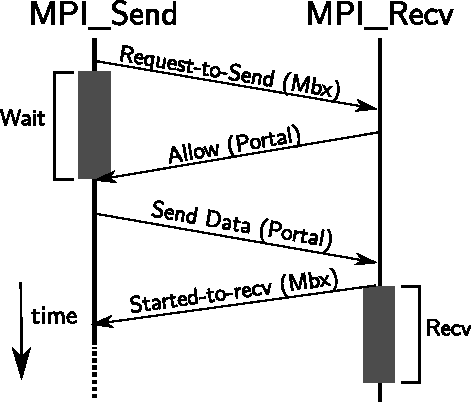
\includegraphics[width=0.55\linewidth]{send-recv_protocol}
		\caption{Communication protocol.}
		\label{figure:comm-protocol}
	\end{figure}

	% Present figures
	Currently, \lwmpi uses the \textit{synchronous mode} to carry out
	communications in \mpisend and \mpirecv functions
	to avoid extra memory usage and keep the library thin (\ie messages
	are not buffered). Figure~\ref{figure:comm-protocol} shows the
	inter-process interaction from the perspective of message exchanges.

	% Send and recv start (steps 1.1 and 2.1)
	Initially, when a \mpisend call is issued, the
	sender builds a request and transfers it to the target process
	using \mailbox, waiting for the receiver to establish the communication.
	The transferred header includes all the information needed by the receiver
	to match a correspondent \mpirecv with the created request, \ie
	communicator id, tag and source/destination.
	%
	At the receiver side, when a \mpirecv call is issued, it looks for a
	matching request that previously arrived or blocks until a matching
	one incomes, if none has been found.

	When a matching request is found, the receiver emits an allow signal
	to the output \portal of the sender, unblocking it and giving permission
	to start the data transfer. The sender, then, starts to send the data
	using the high bandwidth channel. When the receiver starts to receive the
	data in its input \portal, it issues a second started-to-receive signal
	to the sender, signaling that the sender can successfully return when it
	transmitted all the data through the channel.
	%
	The receiver will return from \mpirecv when it has
	read all the data from the channel, or have read the amount of data
	equivalent to the local user buffer size.
               % 2.0 p
\section{Evaluation Methodology}
\label{sec:evaluation-methodology}

	% CAP Benchmark justify
	To deliver a comprehensive assessment of \lwmpi, we relied on a
	subset of the CAP Bench suite~\cite{Souza2017}.
	Applications in CAP Bench are developed in the C language, and feature
	different parallel patterns, task types, communication intensity, and
	task loads. The applications employed in our analysis are:
	%
	\begin{description}
		\item[Friendly Numbers (FN)] is an application that finds all
			subsets of numbers in a range $[n,m]$ that share the same
			\textit{abundance}. The abundance of $n$ is the ratio
			between the sum of divisors of $n$ by $n$ itself. FN
			implements the \textit{MapReduce} parallel pattern and has
			tasks with regular loads. The problem is predominantly
			CPU-bound.

		\item[Gaussian Filter (GF)] is a filter that reduces the noise
			of an image by applying a matrix convolution operation with
			a special two-dimensional Gaussian mask to the image pixels.
			GF performs the \textit{Stencil} parallel pattern to
			equal-sized parts of the image, thus being CPU-intensive and
			having a medium communication intensity.

		\item[K-Means (KM)] is a clustering technique employed in
			data analysis. KM gets a set of $n$ points in real
			$d$-dimensional space and randomly split them into $k$
			partitions. Then, it applies the \textit{Map} parallel
			pattern to distribute points and replicate data centroids
			between the \cclusters. The irregular workload is both CPU-
			and memory-bound. Since each iteration must update data
			centroids, this kernel operates with high communication
			intensity.
	\end{description}

	% Purpose of the kernels' selection 
	We implemented these applications with \mpi\footnote{Publicly
	available at: \url{https://github.com/nanvix/benchmarks}.} and
	contrasted them with the original implementation of the benchmark for
	\mppa. Noteworthy, \textit{a direct performance comparison between these two
	solutions is unfair}, since the original implementation relies on
	a vendor-specific runtime system that is narrowed for
	\mppa but does not provide any means of software portability across
	architectures.

	% Kernels parameters
	Applications in CAP Bench have a single \textit{leader} process that
	coordinates the execution, and may have several \textit{workers}
	that perform the computations.
	%
	Overall, we carried out strong scaling experiments, where we varied
	the number of workers from 1 to 15 and we fixed the problem sizes
	of applications as follows:
	%
	\begin{enumerate*}[label=(\roman*)]
		\item numbers ranging from $1000001$ to $1000129$ for FN;
		\item $512\times512$ image and $7\times$ mask for GF; and
		\item 30720 points and 64 centroids for KM.
	\end{enumerate*}
	%
	We ran 30 trials of each configuration to ensure minimum variance, and
	the maximum coefficient of variance observed was below 1\%.

	%
	% MPPA-256
	\subsection{Experimental Platform}

	The \mppa is an example of an industry-successful lightweight
	manycore, and Figure \ref{figure:lightweight-manycore} presents its
	architectural blueprint.
	%
	Overall, it integrates 288 cores disposed into 20
	clusters. Each cluster is composed of heterogeneous
	hardware capabilities to perform different roles. For instance,
	\ioclusters have four \rmans, four \noc interfaces, and 4~MB local
	\sram to exchange data with external resources and internal clusters.
	Differently, \cclusters have one \rman, 16 \pes, one \noc interface,
	and only 2~MB local \sram to run user workloads. Cores within the
	cluster share and have uniform access to hardware resources.

	% Network-On-Chip
	Communication between clusters is exclusively achieved by explicitly
	exchanging hardware-level messages through two \nocs. Specifically,
	the \cnoc enables synchronization and small control messages handover,
	whereas the \dnoc supports arbitrary-sized data exchanges.
	\ioclusters have direct access to the attached \dram or a device,
	while \cclusters must tile their data into messages and send them
	through the \noc using an \iocluster as an intermediary to access
	these resources. \mppa also features
	a built-in \dma engine in its \noc interfaces to enable asynchronous
	communications and higher bandwidth for dense data transfers.

	\begin{figure}[t]
		\centering
		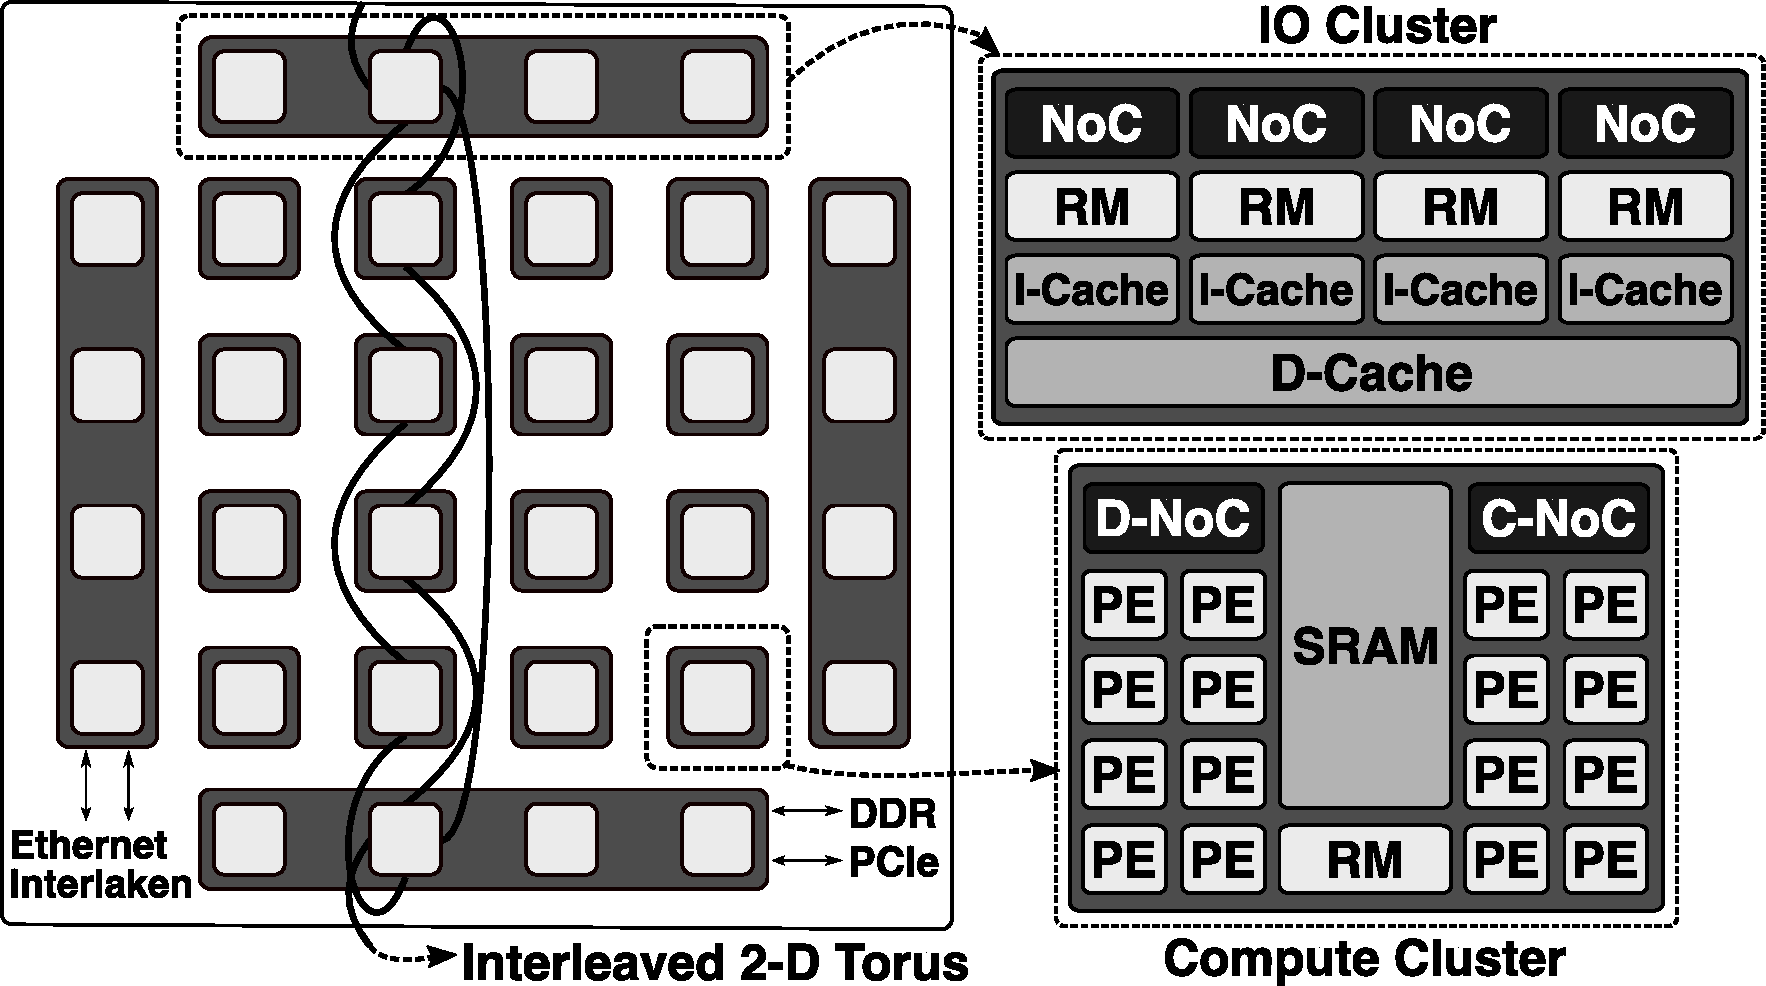
\includegraphics[width=.8\linewidth]{mppa256}
		\caption{\mppa architectural overview.}
		\label{figure:lightweight-manycore}
		\vspace{-10pt}
	\end{figure}
 % 1.0 p
\section{Experimental Results}
\label{sec:experimental-results}
	
	% FN Graphic
	\begin{figure}[t]
		\centering
		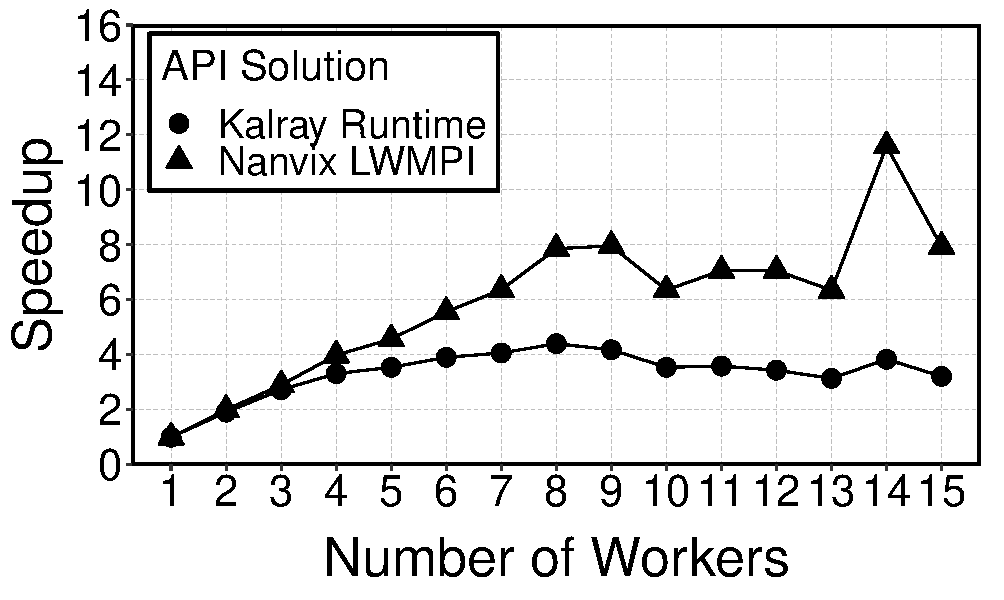
\includegraphics[width=.7\linewidth]{fn-speedup}
		\caption{FN Kernel}
		\label{figure:fn}
		\vspace{-15pt}
	\end{figure}

	\begin{figure}[b]
		\centering
		\vspace{-15pt}
		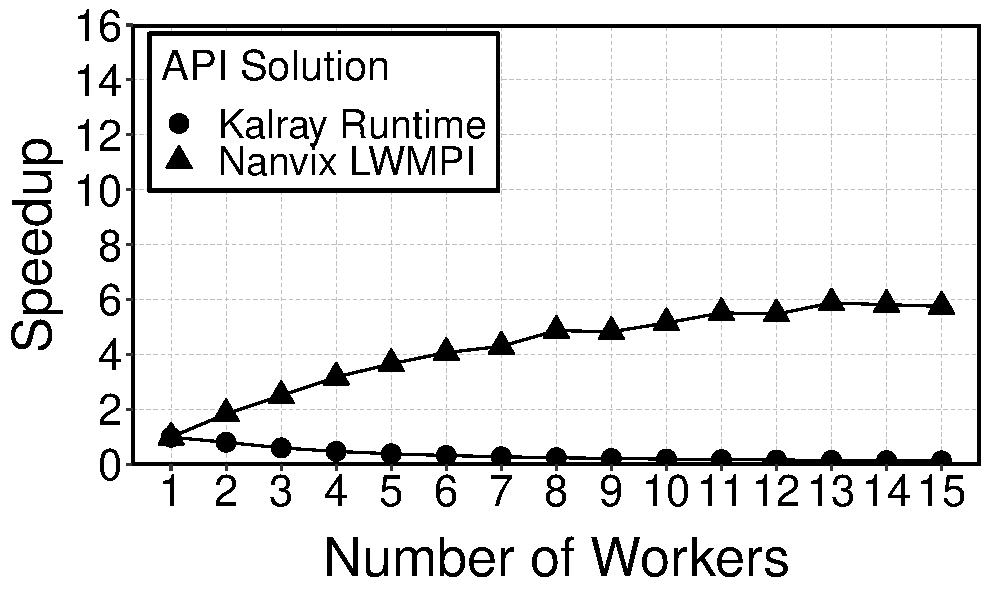
\includegraphics[width=.7\linewidth]{gf-speedup}
		\caption{GF Kernel}
		\label{figure:gf}
	\end{figure}

	% KM Graphic
	\begin{figure}[t]
		\centering
		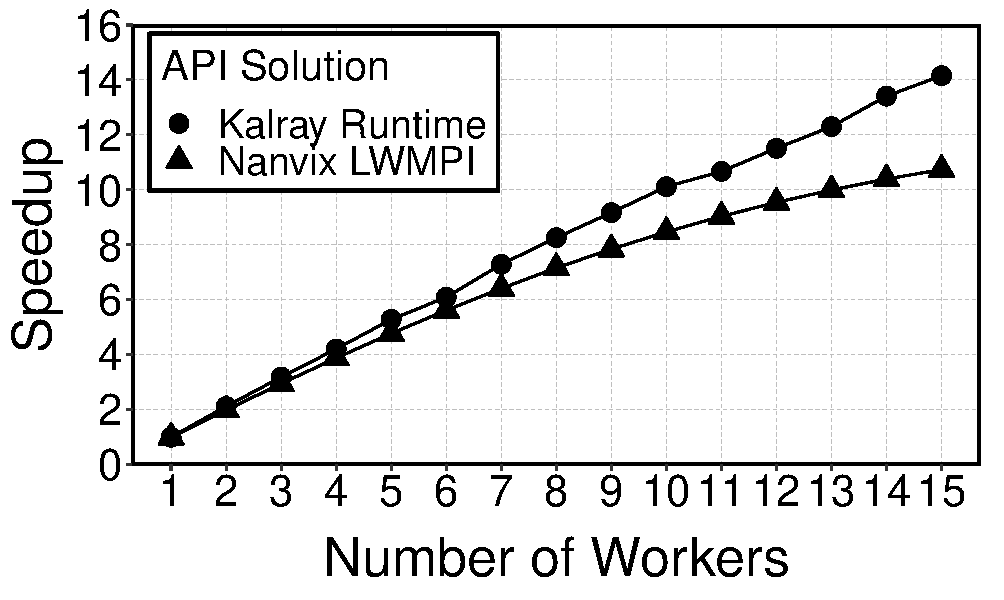
\includegraphics[width=.7\linewidth]{km-speedup}
		\caption{KM Kernel}
		\label{figure:km}
		\vspace{-15pt}
	\end{figure}

	% FN
	% Plot Overview
	Figure~\ref{figure:fn} presents the speedup for the FN application.
	%
	% Plot Analysis
	Since FN is CPU-bound, communication has little interference and
	the results show a similar behavior in both solutions:
	an increase in speedup up to 8 workers and scalability issues, thereafter,
	being the only exception with 14 workers.
	%
	% Additional discussion
	This behavior is due to the problem design itself and the input workload.
	The leader process performs an integer division to compute the minimum amount
	of work to be sent to each worker. Then, the reminder is added to the last worker,
	which may result in load imbalance. This imbalance is very small up to 8 workers,
	but becomes substantial with more workers. With 14 workers, however, the workload
	is well balanced and the overall performance is improved.
	%
	In general, the results show that \lwmpi scaled well and was able to provide an
	easy adaptation of the kernel without introducing an overhead as the parallelism is
	increased.

	% GF 
	% Plot Overview
	Figure~\ref{figure:gf} pictures the speedup for the GF kernel.
	%
	% Plot Analysis
	As it can be noticed, \lwmpi presented suboptimal scalability whereas
	the default runtime library did not scale at all.
	%
	% Additional discussing
	The small problem sizes may have resulted in insufficient workloads,
	deteriorating the performance of the Kalray runtime.
	At the same time, for \lwmpi this problem seems to be attenuated as
	the parallelism increases, proving its scalability also in these
	situations.
	%
	% Possible improvement
	We believe that using asynchronous communications for both
	solutions would significantly reduce the bottleneck on the leader process
	and improve the overall performance.

	% KM
	% Plot Overview
	Figure~\ref{figure:km} shows the speedup for the KM kernel.
	This application has higher communication demands than the
	previous ones, which impacted the results where \lwmpi achieves lower
	speedups when compared to the Kalray runtime.
	%
	% Additional discussion
	This occurred because the baremetal
	runtime can fitly handle the irregular workload, while \lwmpi is
	limited by the coarse-grained fixed-size messages of the
	\portal abstraction in \nanvix.
	Thus, small problem sizes do not overcome the overhead imposed by
	this abstraction, designed to fit dense data transfers.
	%
	% Possible workaround
	Nevertheless, this situation can be settled by a mechanism that dynamically
	chooses which IPC abstraction fits better the data
	granularity to be sent. It would be possible to use the \mailbox
	abstraction to send fine-grained messages and the \portal abstraction for coarse-grained
	ones. As a result, we could transfer small messages with low latency and large messages
	with high bandwidth.
	%
	% Additional Discussion
	Even so, both solutions had similar linear behaviors, showing that
	\lwmpi was able to keep up with the speedup scalability presented by
	the Kalray runtime.

	% Overview
	In general, \lwmpi delivered a lightweight and richer programming
	interface, presenting good scalability for parallel and
	distributed problems.
	%
	% Real contribution
	Consequently, we improve programmability and deliver implicit
	portability for lightweight manycores, which are our main contributions.
   % 2.0 p
\section{Conclusion}
\label{sec:conclusions}

	% Context and problem definition
	Lightweight manycores brought together concepts of parallel and
	distributed systems into a single die to deliver high-performance and
	energy efficiency.  Nevertheless, architectural intricacies and the
	absence of \apis that embrace programmability and portability
	make software development an arduous task, specifically because
	current solutions are hardware-dependent and/or vendor-specific \apis.

	% Goals and contribution
	To unite programmability and portability for \lws,
	we proposed \lwmpi, a lightweight and portable \mpi implementation on
	top of a \posix-compliant distributed \os that targets this class of
	processors. \lwmpi is designed from scratch and follow a two-tier
	approach to separate and self-contain the \mpi interface from the
	\os-dependent layer.
	%
	% Results
	Our experiments on the \mppa processor
	unveil that \lwmpi exposes a richer programming interface and
	achieves similar scalability for parallel and distributed problems, in
	comparison with the vendor-specific \api narrowed for the \mppa.
	%
	% Real contribution
	Thus, the improve in programmability for \lws and the implicit portability
	are our main contributions with \lwmpi.
            % 0.5 p
\section*{Acknowledgements}

	This paper is a simplified version, tailored to the discipline
	"INE410129-41000025DO/ME (2020-1)", of the article entitled "Enhancing Programmability in
	NoC-Based Lightweight Manycore Processors with a Portable MPI Library", presented
	at the XXI Simpósio em Sistemas Computacionais de Alto Desempenho (WSCAD 2020), which also included
	contributions of João V. Souto (UFSC), Pedro H. Penna (PUC-Minas / UGA - France),
	Márcio Castro (UFSC), Henrique Freitas (PUC-Minas) and Jean-F. Méhaut (UGA - France).
      % 0.5 p

\bibliographystyle{IEEEtran}
\bibliography{references.bib}

\end{document}
